\section{Leader Election} % (fold)
\label{sec:leader_election}
As mentioned in section \ref{sec:raft} one of the two main components of Raft is its leader election. The leader election after which the given leader is responsible of replicating commands it receives from a client to the rest of the followers. All servers contain an implementation of Raft, having a log of commands requested by clients. A server can be in three states: leader, candidate or follower.

Figure~\ref{fig:election_example} illustrates the scenario in which a leader is elected:

In the beginning of the illustration, on initial system startup, every server is a follower until $P1$ times out and becomes a candidate. If this candidate receives a majority vote it transitions to the leader state after which it has the leader responsibilities described above. The leader maintains the log matching property by continuously sending empty messages i.e. heartbeats in order to update servers with logs that are not up to date.

\begin{figure}[ht!]
\centering
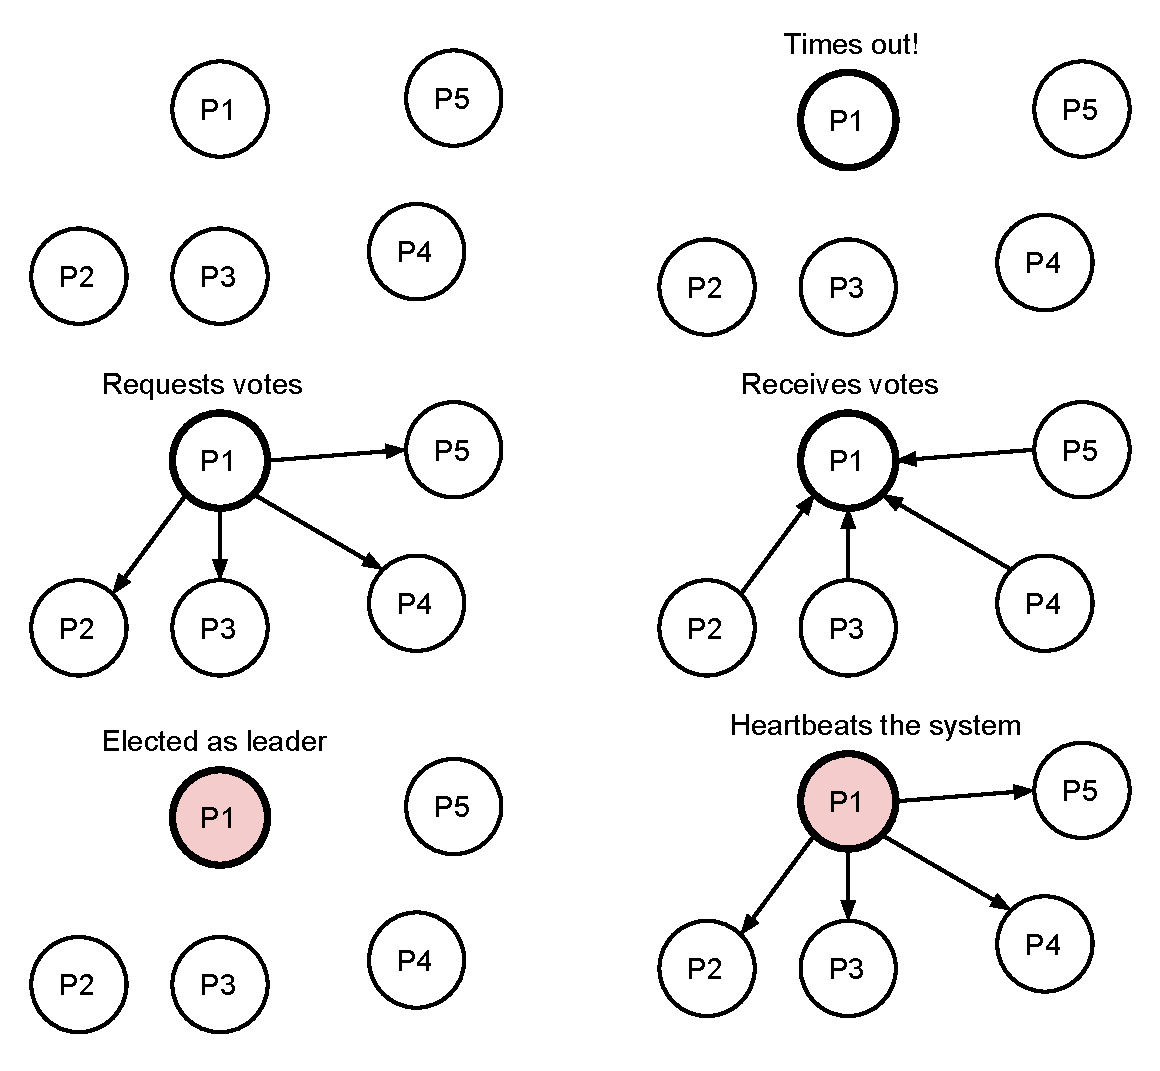
\includegraphics[scale = 0.5]{election-example.pdf}
\caption{A simple scenario where 5 servers are to obtain consensus by first electing a leader.}
\label{fig:election_example}
\end{figure}

Figure~\ref{fig:failure_example} shows how Raft will tolerate a faulty leader. Here we see that the leader $P1$ fails by crashing. $P4$ then times outs and initiates a new election.

\begin{figure}[ht!]
\centering
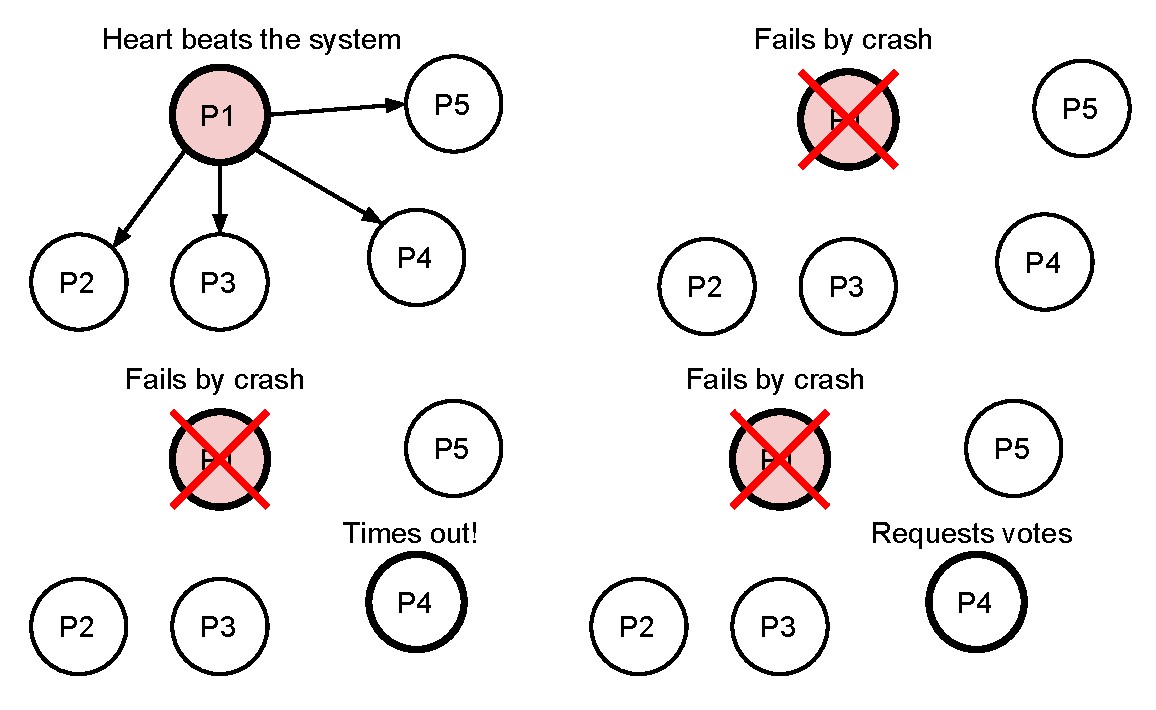
\includegraphics[scale = 0.5]{failure-example.pdf}
\caption{A simple scenario where a leader $P1$ crashes after which $P4$ times out and start a new election.}
\label{fig:failure_example}
\end{figure}

It should also be noted that since the availability, provided by Raft, relies on the majority votes and only non-Byzantine failures, the algorithm can only uphold these properties in a network where $3F \leq N$, where $F$ is the amount of failures and $N$ is the amount of processes in the system.~\cite{Fischer}

Looking back at the Two Generals Problem, Raft is only be able to solve the problem if a majority vote would be possible, which it is not. So in order to solve this problem when utilising Raft, one must add another general to the scenario such that there are an uneven number of generals in the system. We should also modify the problem such that the messenger always tells the truth (i.e. cannot suffer from Byzantine failures). Now that we have three generals and an ``uncapturable'' messenger, they will reach consensus by finding a leader after which he decides when to launch the attack.
% - Theory
% - Analysis
% - Design(?)
    %Vi har egentlig inkoorperet designet givet i Raft paper.
% - Implementation

% section leader_election (end)
